\documentclass[submit]{harvardml}


\course{CS181-S24}
\assignment{Assignment \#1}
\duedate{11:59pm ET, February 10, 2024} 

\usepackage[OT1]{fontenc}
\usepackage[colorlinks,citecolor=blue,urlcolor=blue]{hyperref}
\usepackage[pdftex]{graphicx}
\usepackage{graphicx}
\usepackage{caption}
\usepackage{fullpage}
\usepackage{enumitem}
\usepackage{soul}
\usepackage{amsmath}
\usepackage{amssymb}
\usepackage{color}
\usepackage{todonotes}
\usepackage{listings}
\usepackage{common}
\usepackage{framed}
\usepackage{float}
\usepackage{ifthen}

\usepackage[mmddyyyy,hhmmss]{datetime}

% Solution environment
\newenvironment{solution}
  {\color{blue}\section*{Solution}}
{}

\definecolor{verbgray}{gray}{0.9}

\lstnewenvironment{csv}{
  \lstset{backgroundcolor=\color{verbgray},
  frame=single,
  framerule=0pt,
  basicstyle=\ttfamily,
  columns=fullflexible}}{}

 \DeclareMathOperator*{\limover}{\overline{lim}}


\begin{document}
\begin{center}
{\Large Homework 1: Regression}\\
\end{center}

\subsection*{Introduction}
This homework is on different three different forms of regression:
kernelized regression, nearest neighbors regression, and linear
regression.  We will discuss implementation and examine their
tradeoffs by implementing them on the same dataset, which consists of
temperature over the past 800,000 years taken from ice core samples.

The folder \verb|data| contains the data you will use for this
problem. There are two files:
\begin{itemize}
    \item \verb|earth_temperature_sampled_train.csv| 
    \item \verb|earth_temperature_sampled_test.csv|
\end{itemize} 

Each has two columns.  The first column is the age of the ice core
sample.  The second column is the approximate difference in a year's temperature (K) 
from the average temperature of the 1,000 years preceding it. The temperatures were retrieved from ice cores in
Antarctica (Jouzel et al. 2007)\footnote{Retrieved from
\url{https://www.ncei.noaa.gov/pub/data/paleo/icecore/antarctica/epica_domec/edc3deuttemp2007.txt}

Jouzel, J., Masson-Delmotte, V., Cattani, O., Dreyfus, G., Falourd, 
S., Hoffmann, G., … Wolff, E. W. (2007). Orbital and Millennial 
Antarctic Climate Variability over the Past 800,000 Years. 
\emph{Science, 317}(5839), 793–796. doi:10.1126/science.1141038}.
 
The following is a snippet of the data file:
 
\begin{csv}
# Age, Temperature
399946,0.51
409980,1.57
\end{csv}

\noindent And this is a visualization of the full dataset: 
\begin{center}
  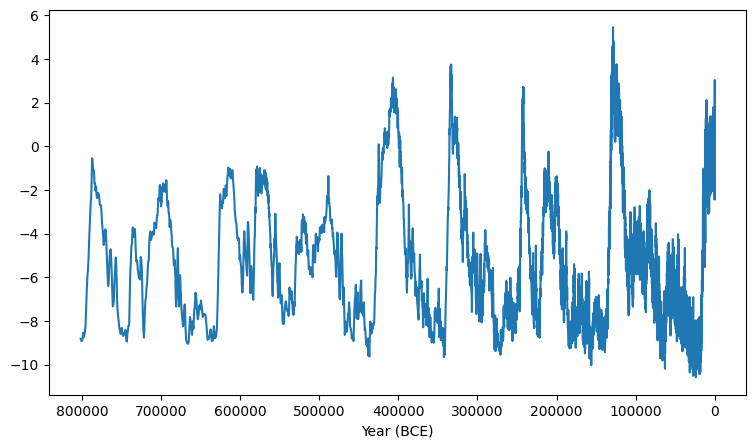
\includegraphics[width=.8\textwidth]{images/sample_graph.png}
    \end{center}
  \noindent 


\textbf{Due to the large magnitude of the years, we will work in terms
  of thousands of years BCE in Problems 1-3.} This is taken care of
for you in the provided notebook.






\subsection*{Resources and Submission Instructions}
If you find that you are having trouble with the first couple
problems, we recommend going over the fundamentals of linear algebra
and matrix calculus (see links on website).  The relevant parts of the
\href{https://github.com/harvard-ml-courses/cs181-textbook/blob/master/Textbook.pdf}{cs181-textbook
  notes are Sections 2.1 - 2.7}.  We strongly recommend reading the
textbook before beginning the homework.

We also encourage you to first read the
\href{http://users.isr.ist.utl.pt/~wurmd/Livros/school/Bishop\%20-\%20Pattern\%20Recognition\%20And\%20Machine\%20Learning\%20-\%20Springer\%20\%202006.pdf}{Bishop
  textbook}, particularly: Section 2.3 (Properties of Gaussian
Distributions), Section 3.1 (Linear Basis Regression), and Section 3.3
(Bayesian Linear Regression). (Note that our notation is slightly
different but the underlying mathematics remains the same!).

\textbf{Please type your solutions after the corresponding problems
  using this \LaTeX\ template, and start each problem on a new page.}
You may find the following introductory resources on \LaTeX\ useful:
\href{http://www.mjdenny.com/workshops/LaTeX_Intro.pdf}{\LaTeX\ Basics}
and
\href{https://www.overleaf.com/learn/latex/Free_online_introduction_to_LaTeX_(part_1)}{\LaTeX\ tutorial
  with exercises in Overleaf}

Homeworks will be submitted through Gradescope. You will be added to
the course Gradescope once you join the course Canvas page. If you
haven't received an invitation, contact the course staff through Ed.

\textbf{Please submit the writeup PDF to the Gradescope assignment
  `HW1'.} Remember to assign pages for each question.

\textbf{Please submit your \LaTeX file and code files to the
  Gradescope assignment `HW1 - Supplemental'.} Your files should be
named in the same way as we provide them in the repository,
e.g. \texttt{hw1.pdf}, etc.


%%%%%%%%%%%%%%%%%%%%%%%%%%%%%%%%%%%%%%%%%%%%%
% Problem 1
%%%%%%%%%%%%%%%%%%%%%%%%%%%%%%%%%%%%%%%%%%%%%
\newpage

\begin{problem}[Setting up the Regression, 10pts]
As noted in the introduction, your goal is to predict temperature
variation given the year.  Before we start deriving and coding up our
regressions, we will interrogate the set-up of our problem.  

\begin{enumerate}
  \item These data were derived from ice core samples in Antarctica.
    Take a brief look at the
    \href{https://www.ncei.noaa.gov/pub/data/paleo/icecore/antarctica/epica_domec/edc3deuttemp2007.txt}{original
      data file}.  Briefly discuss how the data were processed: what kinds of
    decisions and corrections had to be made?  We know that different
    places on earth have different temperatures: what does the
    temperature in the temperature column correspond to?
        
  \item Even before doing any formal regressions, we see that there is
    some periodicity in the data: there are years that are warmer, and
    years that are cooler.  Suppose you are a government official
    advising on how much to worry about climate change.  Would it be
    reasonable to use this pattern as evidence that the earth will
    cool down again?  Why or why not, or to what extent?


  \item In the problems below, we will focus on interpolating
    temperatures for years not provided in the training set.  What
    kind of application would such a regression be useful for?

\end{enumerate}
  
\end{problem}

% qwer
\begin{solution}

\begin{enumerate}
    \item We see that temperature data were corrected for seawater isotopic composition and ice sheet elevation (on the EDC3 age scale), both measures of which were derived from projects by other groups. The temperature in the temperature column is an estimate from the "EPICA Dome C Ice Core, Antarctica (75º 06' S, 123º 21' E)." One very important note: this temperature is a difference from the average temperature of the last 100 years. \\
    
    Additionally, since any measurement cannot be completely accurate due to the limitations of our measurement tools, the researchers say there is an "optimal accuracy of ± 0.5 ‰ (1 sigma), from the surface down to 3259.7 m."\\

    Overall, the researchers had to make decisions while processing the data regarding (1) which scales to use (they are using the EDC3 age scale, for example), (2) which variables they can potentially correct for and whether to correct for those things, and finally, (3) the actual methods of correction. (1) can often be an industry/field standard, but could also definitely vary or change over the years. (2) is limited by the available data, and if researchers use outside data for correction (as was done here) they need to decide whose data to use. (3) could be industry/statistical method standard, but also could be very complex.
    \item It would not be very reasonable to use this pattern as evidence that the earth will cool from modern temperature increases. The temperature estimates are meant to reflect temperatures from $\sim$ 800,000 BCE to 2000 CE, and the world is very different now (e.g. widespread industrialization and climate change since 2000). The researchers have not attempted to control for these changes in environment, so the temperature estimates are not meant to be a reflection of modern temperature patterns.
    \item A regression like this would likely be useful for (1) estimating temperatures in the years soon before/after or within the range of those temperatures in the training set, and (2) estimating temperatures in other years or periods in which we think the relevant environmental factors are similar to those in the training set.
\end{enumerate}
 
\end{solution}
\newpage
% rewq

%%%%%%%%%%%%%%%%%%%%%%%%%%%%%%%%%%%%%%%%%%%%%
% Problem 2
%%%%%%%%%%%%%%%%%%%%%%%%%%%%%%%%%%%%%%%%%%%%%

\begin{problem}[Optimizing a Kernel, 30pts]
Kernel-based regression techniques are similar to nearest-neighbor
regressors: rather than fit a parametric model, they predict values
for new data points by interpolating values from existing points in
the training set.  In this problem, we will consider a kernel-based
regressor of the form:
\begin{equation*}
  f_\tau(x^*) = \cfrac{\sum_{n} K_\tau(x_n,x^*) y_n}{\sum_n K_\tau(x_n, x^*)} 
\end{equation*}
where $\mathcal{D}_\texttt{train} = \{(x_n,y_n)\}_{n = 1} ^N$ are the
training data points, and $x^*$ is the point for which you want to
make the prediction.  The kernel $K_\tau(x,x')$ is a function that
defines the similarity between two inputs $x$ and $x'$. A popular
choice of kernel is a function that decays as the distance between the
two points increases, such as
\begin{equation*}
  K_\tau(x,x') = \exp\left\{-\frac{(x-x')^2}{\tau}\right\}
\end{equation*}
where $\tau$ represents the square of the lengthscale (a scalar value that 
dictates how quickly the kernel decays).  In this
problem, we will consider optimizing what that (squared) lengthscale
should be.

\noindent\emph{Make sure to include all required plots in your PDF.}

\begin{enumerate}
  
\item Let's first take a look at the behavior of the fitted model for different values of $\tau$. Implement the \texttt{kernel\_regressor} function in the notebook, and plot your model for years in the range $800,000$ BC to $400,000$ BC at $1000$ year intervals for the following three values of $\tau$: $1, 50, 2500$. Since we're working in terms of thousands of years, this means you should plot $(x, f_\tau(x))$ for $x = 400, 401, \dots, 800$. \textbf{The plotting has been set up} for you in the notebook already.

Include your plot in your solution PDF.

\textbf{In no more than 5 sentences}, describe how the fits change with $\tau$.

\item Now, we will evaluate the quality of each model \emph{quantitatively} by computing the error on some test set $\mathcal{D}_\texttt{test} = \{(x'_m, y'_m)\}_{m = 1} ^M$.  Write down the expression for MSE of $f_\tau$ over the test set as a function of the training set and test set. Your answer may include $\{(x'_m, y'_m)\}_{m = 1} ^M$, $\{(x_n, y_n)\}_{n = 1} ^N$, and $K_\tau$, but not $f_\tau$.

\item Suppose we used the training set as our test set, that is, we evaluated the expression above with $\mathcal{D}_\texttt{test} = \mathcal{D}_\texttt{train}$, and chose the value of $\tau$ which gave the smallest loss.  What value of $\tau$ would be picked?  Why is setting $\mathcal{D}_\texttt{test} = \mathcal{D}_\texttt{train}$ a bad idea?
   
\emph{Hint: consider what value of $\tau$ would be optimal, for $\tau$ ranging in $(0, \infty)$. We can consider $f_\tau(x^*)$ as a weighted average of the training responses, where the weights are proportional to the distance to $x^*$, and the distance is computed via the kernel. What happens to $K_\tau(x, x')$ as $\tau$ becomes very small, when $x = x'$? What about when $x \neq x'$?}

\item Let us compute the MSE on the provided test set (that is, not the training set). Write Python code to compute the MSE with respect to the same lengthscales as in Part 1. Which model yields the lowest test set MSE? 

\item Describe the time and space complexity of kernelized regression with respect to the size of the training set $N$.  How, if at all, does the size of the model---everything that needs to be stored to make predictions---change with the size of the training set $N$?  How, if at all, do the number of computations required to make a prediction for some input $x^*$ change with the size of the training set $N$?

\end{enumerate}

\end{problem}


% qwer
\begin{solution}
	\begin{enumerate}
    \item Implemented \texttt{kernel\_regressor} function; see notebook.\\

    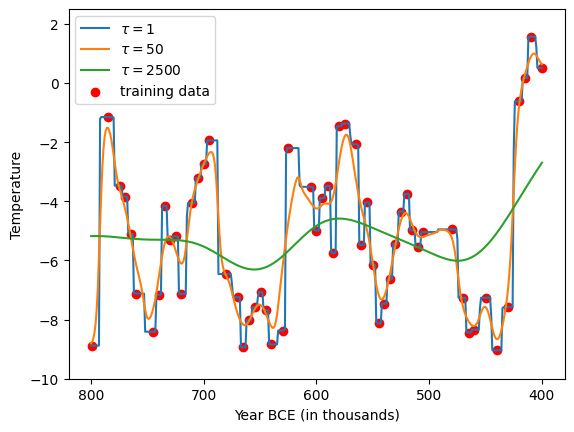
\includegraphics[scale=0.8]{images/p1.2.png}\\
    As $\tau$ increases, the fit becomes increasingly general (i.e. variance decreases), and decreasingly fit to the training data (i.e., bias increases). 
    The higher values of $\tau$ seem to underfit, the lower values of $\tau$ seem to overfit.
    With smaller $\tau$, our predictions deviate much less from the training data, and fit the training data extremely well, but are highly sensitive to any variations in the training data. 
    Meanwhile, with larger $\tau$, our predictions diverge more from the training data, but are more stable/general.
    This is likely because higher $\tau$ gives a smoother kernel with longer lengthscale, which would be directly related to the number of datapoints considered when making each prediction via Kernelized Regression.
    \item We write the MSE of $f_{\tau}$ over the test set as a function of the training set and test set, below:

    \begin{align*}
        \text{MSE}(\{x'_m,y'_m\}_{m=1}^M, \{x_n,y_n\}_{n=1}^N, K_{\tau}) = \frac{1}{M}\sum_{m=1}^M \Bigg(y'_m - \frac{\sum_{n=1}^N K_{\tau}(x_n, x_m')y_n}{\sum_{n=1}^N K_{\tau}(x_n, x'_m)} \Bigg)^2
    \end{align*}
    \item If we used the training set as the test set and chose the $\tau$ that would give us the smallest MSE, we would end up choosing $\tau = 1$. Ultimately our kernel would approximately weight only the given point in our "prediction", yielding a "prediction" extremely close to or exactly the same as the $y$ value in our original data (the only reason it may not be exactly the same is that the kernel may be defined in such a way that even using the minimum bandwidth of 1 allows for other points to be very weakly weighted in the prediction).\\
    We show that the kernel would make this prediction using the MSE equation:
    \begin{align*}
        \text{MSE}(\{x'_m,y'_m\}_{m=1}^M, \{x_n,y_n\}_{n=1}^N, K_{\tau}) = \frac{1}{M}\sum_{m=1}^M \Bigg(y'_m - \frac{\sum_{n=1}^N K_{\tau}(x_n, x_m')y_n}{\sum_{n=1}^N K_{\tau}(x_n, x'_m)} \Bigg)^2
    \end{align*}
    To minimize this MSE, we want our predicted value  $\frac{\sum_{n=1}^N K_{\tau}(x_n, x_m')y_n}{\sum_{n=1}^N K_{\tau}(x_n, x'_m)}$ to be as close to $y'_m$ as possible. This forces $\tau$ to the minimum value $\tau = 1$ so that we weight the input point as much as possible and the rest of the points as little as possible.\\
    
    We know this would minimize MSE since for any $(x_n, y_n)$, $(x'_m, y'_m) = (x_n, y_n)$ at some point during our MSE calculation and there are no other points in the test set we need to consider that would contribute to MSE.\\

    Now with the choice of $\tau = 1$, we see that with our choice of kernel $K_1(x, x') = \frac{1}{exp\{(x-x')^2\}}$. So, if $x = x'$, this value is equal to 1; otherwise it is approximately 0. We now know that the kernel in this training data = testing data scenario will only weight each reappearing training point in its prediction (with some mild potential divergence from extremely low weights on nearby points).\\

    \textbf{Ultimately, this is a poor idea because it is not a meaningful regression.} We get no new information this way and only reproduce the exact original data, leading to a regression with very low bias but the same variance as the original data.
     
    \item Implemented MSE computation; see notebook.\\

    tau = 1: loss = 1.9472621565209178\\
tau = 50: loss = 1.8582899169613447\\
tau = 2500: loss = 8.333886806980791\\

    The model with $\tau=50$ gives us the lowest test set MSE.
    \item The \textbf{time complexity} of Kernelized regression is $O(N)$. To predict one $x*$ value, we must compute the $K_{\tau}$ calculation and multiply by $y_n$ for all $x_n$ for $n \in [1,N]$, which takes approximately $O(3N) = O(N)$. From there we compute the sum of $n$ terms which also takes $O(N)$, to achieve the numerator. For the denominator, we must compute $K_{\tau}$ $N$ times for each $x_n$ for $n \in [1,N]$, then compute the sum of these $N$ terms, so this is also approximately $O(2N) = O(N)$. Altogether we have $O(5N) = O(N)$ time complexity.\\

    The \textbf{space complexity} of Kernelized regression is $O(N)$ since it must store the $N$ size training dataset.
 \end{enumerate}
\end{solution}
% rewq

%%%%%%%%%%%%%%%%%%%%%%%%%%%%%%%%%%%%%%%%%%%%%
% Problem 3
%%%%%%%%%%%%%%%%%%%%%%%%%%%%%%%%%%%%%%%%%%%%%

\newpage
\begin{problem}[Kernels and kNN, 20pts]

Now, let us compare the kernel-based approach to an approach based on
nearest-neighbors.  Recall that kNN uses a predictor of the form
  \begin{equation*}
    f(x^*) = \frac{1}{k} \sum_n y_n \mathbb{I}(x_n \texttt{ is one of k-closest to } x^*)
  \end{equation*}

\noindent where $\mathbb{I}$ is an indicator variable. For this problem, you will use the \textbf{same dataset as in Problem 1}.


%\textbf{For this problem, you may also use the second half of the notebook at {\color{red} update name} \texttt{T1\_P1-2.ipynb}.} 

\textbf{Note that our set of test cases is not comprehensive: just because you pass does not mean your solution is correct! We strongly encourage you to write your own test cases and read more about ours in the comments of the Python script.}

\vspace{0.5cm}
\noindent\emph{Make sure to include all required plots in your PDF.}


\begin{enumerate}

\item The kNN implementation \textbf{has been provided for you} in the notebook. Run the cells to plot the results for $k=\{1, 3, N-1\}$, where $N$ is the size of the dataset.

  Describe what you see: what is the behavior of the functions in
  these three plots?  How does it compare to the behavior of the
  functions in the three plots from Problem 1? In particular, are
  there situations in which kNN and kernel-based regression
  interpolate similarly?

\item Compute the MSE on the test set for each value of $k$.  Which solution has the lowest MSE?  

\item As in Problem 1, describe the space and time complexity of kNN.  How does what is stored to compute predictions change with the size of the training set $N$?  How does the computation needed to compute the prediction for a new input depend on the size of the training set $N$? (For the latter, justify based off of your implementation.)

\end{enumerate}

\end{problem}


% qwer
\begin{solution}

% n-1 is super close to just to just the average
\begin{enumerate}
    \item 
    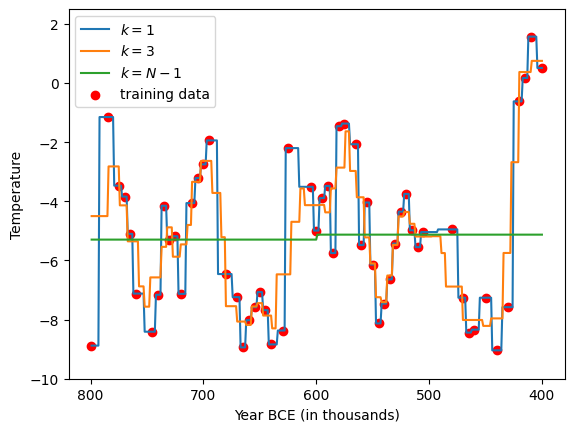
\includegraphics[scale=0.8]{images/p2.1.png}\\
    As $k$ increases, we observe that variance seems to decrease and bias seems to increase. The higher values of $k$ seem to underfit, the lower values of $k$ seem to overfit. In other words, as $k$ increases, the sensitivity of our predictions to the training data seems to decrease and the amount our predictions diverge from the training data seems to increase. 
    This has a similar effect to when we increased $\tau$ in problem 2. Increasing $k$ seems to have a similar effect to increasing $\tau$ where individual predictions would become reliant on more datapoints. In $k$ NN this reliance/\# datapoints considered increases deterministically since this is just $k$, but in kernelized regression the increase in reliance to other datapoints may vary based on the shape of the data.
    \item Implemented MSE computation; see notebook.\\

    k = 1: MSE loss = 1.7406000000000004\\
k = 3: MSE loss = 3.890766222222223\\
k = 56: MSE loss = 9.528571442602042\\
k = 57: MSE loss = 9.578326603878116\\

    The model with $k=1$ gives us the lowest test set MSE.
    \item The \textbf{time complexity} is $O(N\log N)$. To make each prediction, we must sort the data, which takes $O(N\log N)$, in order to find the nearest neighbors. Then we take $O(N)$ operations to take the mean of the nearest neighbors' values. 

    The \textbf{space complexity} is $O(N)$ since we must store the entire training dataset to make predictions.
\end{enumerate}
\end{solution}
% rewq


%%%%%%%%%%%%%%%%%%%%%%%%%%%%%%%%%%%%%%%%%%%%%
% Problem 4
%%%%%%%%%%%%%%%%%%%%%%%%%%%%%%%%%%%%%%%%%%%%%

\newpage
\begin{problem}[Modeling Climate Change 800,000 Years Ago, 30pts]

Our last regression will be linear regression.  We currently only have
a one dimensional input, the year.  To create a more expressive linear
model, we will introduce basis functions.
\vspace{1em}
\noindent\emph{Make sure to include all required plots in your PDF.}

\begin{enumerate}
\item 
We will first implement the four basis regressions below. (The first basis has been implemented for you in the notebook as an example.) Note that we introduce an addition transform $f$ (already into the provided notebook) to address concerns about numerical instabilities.
\begin{enumerate}
  \item $\phi_j(x)= f(x)^j$ for $j=1,\ldots, 9$. $f(x) = \frac{x}{1.81 \cdot 10^{2}}.$
  \item $\phi_j(x) = \exp\left\{-\cfrac{(f(x)-\mu_j)^2}{5}\right\}$ for $\mu_j=\frac{j + 7}{8}$ with $j=1,\ldots, 9$. $f(x) = \frac{x}{4.00 \cdot 10^{2}}.$
  \item $\phi_j(x) =  \cos(f(x) / j)$ for $j=1, \ldots, 9$. $f(x) = \frac{x}{1.81}$.
  \item $\phi_j(x) = \cos(f(x) / j)$ for $j=1, \ldots, 49$. $f(x) = \frac{x}{1.81 \cdot 10^{-1}}$. \footnote{For the trigonometric bases (c) and (d), the periodic nature of
cosine requires us to transform the data such that the 
lengthscale is within the periods of each element of our basis.}
\end{enumerate}

{\footnotesize * Note: Please make sure to add a bias term for
all your basis functions above in your implementation of the 
\verb|make_basis|.}

Let 
$$ \mathbf{\phi}(\mathbf{X}) = 
\begin{bmatrix} 
\mathbf{\phi}(x_1) \\
\mathbf{\phi}(x_2) \\
\vdots \\
\mathbf{\phi}(x_N) \\
\end{bmatrix} \in \mathbb{R}^{N\times D}.$$
You will complete the \verb|make_basis| function which must return
$\phi(\mathbf{X})$ for each part 
(a) - (d). You do NOT need to submit this
code in your \LaTeX writeup.

For each basis create a plot of your code graphing the least squares
regression line trained on your training data against a scatter plot
of the training data. Boilerplate plotting code is provided in the
notebook.
\textbf{All you need to include 
in your writeup for this part are these four plots.}
\vspace{1em}
\end{enumerate}
\end{problem}


\newpage
\begin{framed}
\noindent\textbf{Problem 4} (cont.)\\
\begin{enumerate}
\setcounter{enumi}{1}
\item 
Now we have trained each of our basis regressions.  For each basis
regression, compute the MSE on the test set.  Discuss: do any of the
bases seem to overfit?  Underfit?  Why?

% \item Make a claim regarding whether this basis overfits, 
% underfits, or fits well. Write 1-2 sentences explaining your 
% claim using the train and test negative log-likelihood and MSE.

% \end{itemize}

\item Briefly describe what purpose the transforms $\phi$ serve: why are they helpful?

\item As in Problems 1 and 2, describe the space and time complexity of linear regression.  How does what is stored to compute predictions change with the size of the training set $N$?  How does the computation needed to compute the prediction for a new input depend on the size of the training set $N$?  How do these complexities compare to those of the kNN and kernelized regressor?

\item Briefly compare and constrast the different regressors: kNN,
  kernelized regression, and linear regression (with bases).  Are some
  regressions clearly worse than others?  Is there one best
  regression?  How would you use the fact that you have these multiple
  regression functions?
  
\end{enumerate}
Note:
Recall that we are using a 
different set of inputs $\mathbf{X}$ for each basis (a)-(d). 
Although it may seem as though this prevents us from being able 
to directly compare the MSE since we are using different data, 
each transformation can be considered as being a part of our model. 
Contrast this with transformations (such as standardization) that cause the variance of the target $\mathbf{y}$ to be different; in these cases the
MSE can no longer be directly compared.

\end{framed}

% qwer
\begin{solution}
\begin{enumerate}
    \item 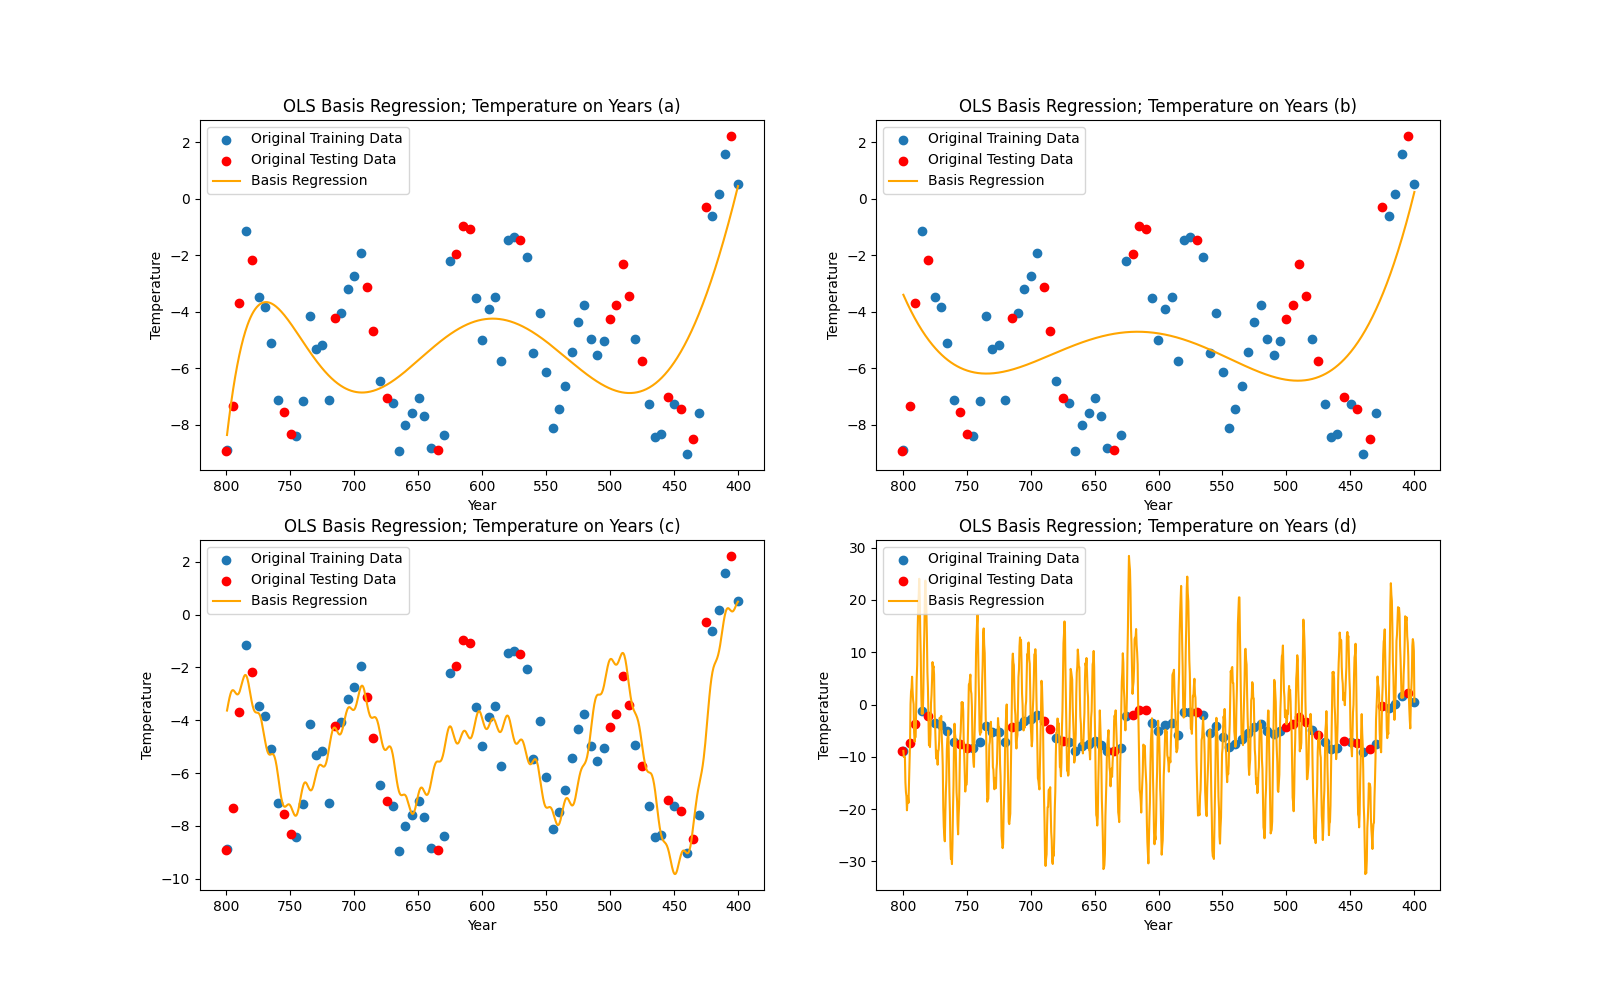
\includegraphics[scale=0.4]{images/p3.1.png}
    \item 

\subsection*{Results}
    Part (a);

 Train MSE: 4.82; Test MSE: 7.96


Part (b);

 Train MSE: 5.53; Test MSE: 8.71


Part (c);

 Train MSE: 2.88; Test MSE: 5.97


Part (d);

 Train MSE: 0.64; Test MSE: 58.92
    
\subsection*{Analysis}
    
    All of the bases seem to overfit to some extent, as train MSE $<$ test MSE for all of the bases. In order, the severity of the overfit (test MSE - train MSE) is: (d) $>>$ (b) $>$ (a) $>$ (c), with (a), (b), and (c) all overfitting to a similar severity (at least, going by my naive way of estimating severity, test MSE - train MSE).\\

    Thinking more about the basis transforms to consider why they overfit (and to these different extents), we look at the plots and the math of the basis transforms themselves.\\
    
    We can see from the plots and regressions using each basis that (d)'s regression line has a high variance and very low bias — it technically hits all of the training points, but produces a pattern that seems inaccurate to the whole dataset.\\

    Meanwhile (a) and (b) produce lines with relatively high train MSE. We can see from the graph that these regressions have higher bias. But this comes at the tradeoff of low variance, which enables a more general fit on the test set.\\

    Lastly, (c) seems to strike a happy medium in the bias-variance tradeoff with the lowest MSE on both train and test datasets.\\

    Why might this occur mathematically? I propose this is due to the appropriateness of the basis transform for the shape of the data. The data seems roughly periodic, and the basis transforms of (a) and (b) do not seem to capture the periodic nature. Meanwhile, the basis transform of (d) is periodic, but the amplitude in the period appears far too large. The basis transform of (c) likely accurately captures the periodic shape of the data.
    
    \item The basis transforms account for the nonlinear shape of the data. The data is periodic, and the basis transforms aim to capture this using a nonlinear equation. Once we apply the basis transforms, we can fit a linear regression to the transformed (originally nonlinear values) and the weights, meaning that in effect the basis regression is only linear in the weights.
    
    \iffalse Attempting the basis regressions without the $f$ transforms (as an experiment), I observe that the basis regression lines look far more unstable in relation to the data. It seems like the $f$ transforms are helpful to prevent higher or lower values from "exploding" the basis transform. \\
    
    Since the (a) basis transform involves exponentiation, using $f$ to transform the wide range of years approximately ranging from $[400,800]$ BCE is important to make sure the exponent doesn't take on extreme values.\\

    On the other hand, since the (b) basis transform uses its input values in a negative exponent of $e$, without scaling with $f$, all of the values would be extremely close to 0.\\

    The (c) and (d) $f$ transforms seem not to matter as much because of the periodic nature of the cosine function basis transform, meaning that values won't "explode." The transforms are likely in place to keep a reasonable amplitude. \fi 
    
    \item The \textbf{time complexity} to make a new prediction for a linear regression is $O(D)$ where $|w| = D$, since we only need multiply the inputs by the weights. The \textbf{space complexity} is also $O(D)$ since we need only store the weights after computing them.
    
    \item The key difference between the nonparametric regressions ($k$NN, kernelized) and parametric regression (linear regression) seems to be that in the linear regrssion we can "throw away" the training data and just retain the weights, which is much more lightweight and performant, with potential huge gains for space and time performance if datasets are large.\\
    
    However, the regressions vary in ease of customizability. It is easy to customize the fit of $k$NN and Kernelized regression to manage the bias-variance tradeoff and observe how different values of $k$ or Kernels lead to overfitting, underfitting, or a proper fit. But the main way to customize a linear regression is via basis transformation, which is harder and relies on fitting a potentially complex nonlinear function to the data — there is a lot of poetntial for over/underfitting from a basis function/set of bases that is too/not complex enough.\\

    Of the nonparametric regressions, kernelized regression seems better if we are confident in our choice of kernel and don't have a reasonable notion of similarity/distance for our dataset. \\
    
    On the other hand, if we are using Euclidean distance and find that our data doesn't tend to form, e.g. clusters that are wildly far from each other (which would lead to "wrong neighbors" potentially being included in $k$NN) $k$NN may be a better choice.\\

    Overall, linear regression is better in terms of performance and space concerns but is harder to customize the fit for. Kernelized regression and $k$NN could be good choices if performance and space are not pressing concerns; between those two, one regression is not better than the other. The choice of kernel and the choice of $k$ are very important considerations that strongly impact the fit of the regression, as we have seen. 
    
    \end{enumerate}
\end{solution}
% rewq

%%%%%%%%%%%%%%%%%%%%%%%%%%%%%%%%%%%%%%%%%%%%%
% Problem 5
%%%%%%%%%%%%%%%%%%%%%%%%%%%%%%%%%%%%%%%%%%%%%
\newpage
\begin{problem}[Deriving Linear Regression, 10pts]

  In the previous problems, you focused on implementing regressions
  and exploring their fits on data. Now we will turn to some more
  analytic work.  Specifically, the solution for the least squares
  linear regressions ``looks'' kind of like a ratio of covariance and
  variance terms.  In this problem, we will make that connection more
  explicit. \\

  \noindent Let us assume that our data are tuples of scalars $(x,y)$ that are
  described by some joint distribution $p(x,y)$.  For clarification, the joint distribution $p(x,y)$ is just another way of saying the ``joint PDF'' $f(x,y)$, which may be more familiar to those who have taken Stat 110, or equivalent. \\
  
  \noindent We will consider the process of fitting these data from this distribution with the best linear model
  possible, that is a linear model of the form $\hat{y} = wx$ that
  minimizes the expected squared loss $E_{x,y}[ ( y - \hat{y} )^2
  ]$.\\

\noindent \emph{Notes:} The notation $E_{x, y}$ indicates an
expectation taken over the joint distribution $p(x,y)$.  Since $x$ and
$y$ are scalars, $w$ is also a scalar.
  
  \begin{enumerate}

  \item Derive an expression for the optimal $w$, that is, the $w$
    that minimizes the expected squared loss above.  You should leave
    your answer in terms of moments of the distribution, e.g. terms
    like $E_x[x]$, $E_x[x^2]$, $E_y[y]$, $E_y[y^2]$, $E_{x,y}[xy]$
    etc.

\item Provide unbiased and consistent formulas to estimate $E_{x, y}[yx]$
 and $E_x[x^2]$ given observed data $\{(x_n,y_n)\}_{n=1}^N$.

\item In general, moment terms like $E_{x, y}[yx]$, $E_{x, y}[x^2]$,
  $E_{x, y}[yx^3]$, $E_{x, y}[\frac{x}{y}]$, etc. can easily be
  estimated from the data (like you did above).  If you substitute in
  these empirical moments, how does your expression for the optimal
  $w^*$ in this problem compare with the optimal $w^*$ that we see in
  Section 2.6 of the cs181-textbook?

\item Many common probabilistic linear regression models assume that
  variables x and y are jointly Gaussian.  Did any of your above
  derivations rely on the assumption that x and y are jointly
  Gaussian?  Why or why not?
    
\end{enumerate}
  
\end{problem}

\begin{solution}
\begin{enumerate}
    \item We first take the derivative of the expression for expected squared loss below:

    \begin{align*}
    L(x,y) = E_{x,y}[(y-wx)^2] \\
    = E_{x,y}[(y^2 - 2wxy + w^2x^2)] \\
    \frac{\partial L(x,y)}{\partial w} = -2E_{x,y}[xy] + 2wE_x[x^2] 
    \end{align*}

    We now set this derivative equal to 0 to find the optimal weights minimizing loss, which we denote $w*$:
    \begin{align*}
    -2E_{x,y}[xy] + 2w*E_x[x^2]  = 0\\
     2w*E_x[x^2] = 2E_{x,y}[xy]\\
     w* = \frac{E_{x,y}[xy]}{E_x[x^2]}
    \end{align*}
    \item To estimate $E_{x, y}[yx]$
 and $E_x[x^2]$ given observed data $\{(x_n,y_n)\}_{n=1}^N$, we use Method of Moments estimators and substitute in the sample moments. We denote these estimators as $\hat{E_x[x^2]}$ and $\hat{E_{x,y}[xy]}$ respectively.

 \begin{align*}
     \hat{E_x[x^2]} = \frac{1}{N}\sum_{n=1}^N (x_n)^2\\
     \hat{E_{x,y}[xy]} = \frac{1}{N} \sum_{n=1}^N x_ny_n
 \end{align*}
    \item Substituting in the empirical moments, we get:
    \begin{align*}
        w* = \frac{\frac{1}{N} \sum_{n=1}^N x_ny_n}{\frac{1}{N}\sum_{n=1}^N (x_n)^2}\\
        = \frac{\sum_{n=1}^N x_ny_n}{\sum_{n=1}^N (x_n)^2}
    \end{align*}
    In the textbook, we find the equation:
    \begin{align*}
        w* = (X^TX)^{-1}X^TY
    \end{align*}
    Which uses $X$ to represent the sample $x_n$ values in the training data as a matrix, and $Y$ to represent the sample $y_n$ values in the training dataset as a vector. Interpreting the matrix multiplication, we see that these are essentially the same. Taking the inverse of the $X^TX$ matrix product and multiplying this by the $X^TY$ matrix product yields the same calculations: $\frac{\sum_{n=1}^N x_ny_n}{\sum_{n=1}^N (x_n)^2}$.
    \item When taking the expected values using the joint PDFs or using the Method of Moments estimator, we never assumed that $X,Y$ are jointly Gaussian. This is because the probabilistic approach we took to find our weights, i.e. using the Method of Moments, is nonparametric — taking the empirical moments does not assume any distribution in particular.
\end{enumerate}
\end{solution}

%%%%%%%%%%%%%%%%%%%%%%%%%%%%%%%%%%%%%%%%%%%%%
% Name and Calibration
%%%%%%%%%%%%%%%%%%%%%%%%%%%%%%%%%%%%%%%%%%%%%
\newpage
\subsection*{Name}

\subsection*{Collaborators and Resources}
Whom did you work with, and did you use any resources beyond cs181-textbook and your notes?

Collaborators: Teresa Lu-Romeo, Jodie Kuo, Karen Song


\end{document}
